\chapter{Batteries and Circuits}

\section{Batteries}

\subsection{EMF: Electromotive Force}

\begin{definition}[EMF]
The electromotive force (EMF) is defined as the line integral of the electric field from the negative terminal to the positive terminal:
\[
    \mathcal{E} = \int_{+\,\text{terminal}}^{-\,\text{terminal}} \vect{E}\cdot d\vect{s} = \text{EMF}
\]
\end{definition}

EMF is the work per unit charge done by non-electrostatic forces (chemical, mechanical) around a circuit. It drives current against the resistance of the circuit. A battery maintains a potential difference by doing chemical work on charges, transporting them from low to high potential inside the cell.

\section{Circuits}

\subsection{Kirchhoff's Rules}

\begin{theorem}[Kirchhoff's Voltage Law (Rule 2)]
The sum of EMFs and potential drops around any closed loop must add up to zero. This comes from the fact that $\oint \vect{E}\cdot d\vect{s} = 0$ for the electrostatic field — equivalently, energy is conserved around any loop.
\[
    \mathcal{E} = IR
\]
\end{theorem}

\subsection{Resistors in Series}

For two resistors $R_1$ and $R_2$ in series, by Kirchhoff's voltage law:
\[
    -\mathcal{E} + IR_1 + IR_2 = 0
\]
\[
    \Rightarrow \quad I = \frac{\mathcal{E}}{R_1 + R_2}
\]

Resistors in series add up: $R_\text{eff} = R_1 + R_2$.

\subsection{Resistors in Parallel}

\begin{theorem}[Kirchhoff's Current Law (Rule 1)]
At any current junction: $I = I_1 + I_2$. This follows from charge conservation: in steady state $\div\vect{J}=0$, so no charge accumulates at a node.
\end{theorem}

Using the first rule:
\begin{align*}
    -\mathcal{E} + I_1 R_1 &= 0 \quad\Rightarrow\quad I_1 = \mathcal{E}/R_1 \\
    -\mathcal{E} + I_2 R_2 &= 0 \quad\Rightarrow\quad I_2 = \mathcal{E}/R_2
\end{align*}

Thus:
\[
    I = \mathcal{E}\!\left(\frac{1}{R_1} + \frac{1}{R_2}\right)
\]
\[
    \Rightarrow \quad \mathcal{E} = I\!\left(\frac{1}{\frac{1}{R_1}+\frac{1}{R_2}}\right)
    = I\!\left(\frac{R_1 R_2}{R_1+R_2}\right) \quad \leftarrow R_\text{parallel}
\]

Voltage divider output:
\[
    V_\text{out} = \frac{R_2}{R_1+R_2}\,V_\text{in}
\]

\subsection{Energy Dissipation}

\[
    dW = V\,dq
\]

Power:
\[
    P = \frac{dW}{dt} = V\frac{dq}{dt} = VI = \boxed{I^2 R} = \frac{V^2}{R}
\]

\section{Linearity of DC Networks}

\begin{fact}[Superposition in DC networks]
Because the voltages and currents are governed by linear equations, a superposition of possible states of the network (a set of currents and potentials $V_1,\ldots,V_n$, $I_1,\ldots,I_m$) is also a solution ($V_1+V_1', I_1+I_1'$, etc.).
\end{fact}

\section{Energy Dissipation in Current Flow}

The power delivered to push a charge through a field $\vect{E}$ is $q\vect{E}\cdot\vect{v}$, and this energy is ultimately transferred to heat via lattice collisions. For a current $I$ through a resistor $R$ at voltage $V$, the net work done in $\Delta t$ is:
\[
    q_\text{total}\,\Delta\phi = (I\,\Delta t)\,V - I^2 R\,\Delta t
    \quad\Rightarrow\quad \boxed{\frac{dW}{dt} = I^2 R = P}
\]

(Units: 1 watt $= 1\;\text{joule/second}$)

\section{Electromotive Force and Voltaic Cells}

EMF transports charge carriers in the \emph{opposite} direction to what the electric field alone would drive them. In a Van de Graaff generator, mechanical work cranks charges up the shaft to potential $V_0$; in a battery, charge carriers move to higher energy because doing so releases more chemical energy than it costs.

\subsection{Example: Voltaic Cells}

A voltaic cell is a chemical source of EMF; the lead-sulfuric acid cell is a classic example in which redox reactions drive charge separation between the electrodes.

\section{Networks with Voltage Sources}

\subsection{Applying Kirchhoff's Rules}

\begin{example}[Multi-loop network]
Consider a circuit with EMFs $\mathcal{E}_1$, $\mathcal{E}_2$ and resistors $R$, $R_2$, $R_3$, and currents $I_1$, $I_2$, $I_3$. The equations from Kirchhoff's rules are:
\begin{align*}
    I_1 &= I_2 + I_3 \\
    \mathcal{E}_1 - I_1 R_1 - I_3 R_3 &= 0 \\
    I_3 R_3 - I_2 R_2 + \mathcal{E}_2 &= 0
\end{align*}
\end{example}

Using the more efficient loop-current method:
\begin{align*}
    \mathcal{E}_1 - R_1 I_1 - R_3(I_1 - I_2) &= 0 \\
    \mathcal{E}_2 - R_3(I_2 - I_1) - R_2 I_2 &= 0
\end{align*}

The result is:
\[
    I_1 = \frac{\mathcal{E}_1 R_2 + \mathcal{E}_1 R_3 + \mathcal{E}_2 R_3}{R_1 R_2 + R_2 R_3 + R_1 R_3}
\]
\ldots etc., used with a linear algebra solver. The second method is usually more tractable.

\section{Thevenin's Theorem}

\begin{theorem}[Thevenin's Theorem]
Any two-terminal ``black box'' circuit (no matter how complicated) is equivalent to a resistor $R_\text{eq}$ and a battery $\mathcal{E}_\text{eq}$ in series.
\end{theorem}

If we don't know what is in the box, we determine $\mathcal{E}_\text{eq}$ and $R_\text{eq}$ by measuring the open-circuit voltage between A and B (which equals $\mathcal{E}_\text{eq}$) and the short-circuit current through an ammeter of negligible resistance:
\[
    \boxed{R_\text{eq} \cong \frac{\mathcal{E}_\text{eq}}{I_\text{eq}}}
\]

\subsection{If We Do Know the Box}

Calculate $\mathcal{E}_\text{eq}$ ($= V_\text{TH}$) as the open-circuit voltage at A and B with the load removed. For $R_\text{eq}$, either short the terminals and compute $I_\text{sc}$ (then $R_\text{eq} = \mathcal{E}_\text{eq}/I_\text{sc}$), or zero all internal EMFs (remove batteries) and compute the resistance seen at the port directly.

\section{Variable Currents in Capacitors and Resistors}

Consider an $RC$ circuit (resistor $R$ and capacitor $C$ in series with EMF $\mathcal{E}$):
\[
    Q = CV, \qquad I = \frac{V}{R}, \qquad I = -\frac{dQ}{dt}
\]

\begin{figure}[H]
\begin{center}
\begin{tikzpicture}[scale=0.95]
  % RC circuit schematic
  \draw (0,2) to[battery1, l=$\mathcal{E}$] (0,0);
  \draw (0,2) to[R, l=$R$] (2.5,2);
  \draw (2.5,2) to[C, l=$C$] (2.5,0);
  \draw (0,0) -- (2.5,0);
  % Current arrow
  \draw[-{Stealth[length=5pt]}, thick, red!70!black]
    (0.3,2.15) -- (1.0,2.15) node[above]{$I$};
  % Voltage labels
  \node[right, font=\small] at (2.7,1.0) {$V_C$};
\end{tikzpicture}
\hspace{1.5cm}
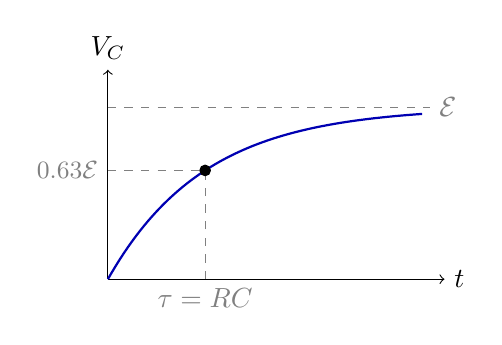
\begin{tikzpicture}[scale=0.95]
  % V_C vs time: charging curve
  \draw[->] (0,0) -- (4.5,0) node[right]{$t$};
  \draw[->] (0,0) -- (0,2.8) node[above]{$V_C$};
  \draw[dashed, gray] (0,2.3) -- (4.3,2.3) node[right]{$\mathcal{E}$};
  \draw[thick, blue!70!black, domain=0:4.2, samples=80]
    plot (\x, {2.3*(1 - exp(-\x/1.3))});
  % tau marker
  \draw[dashed, gray] (1.3,0) node[below]{$\tau=RC$} -- (1.3,{2.3*(1-exp(-1))});
  \draw[dashed, gray] (0,{2.3*(1-exp(-1))}) node[left, font=\small]{$0.63\mathcal{E}$}
    -- (1.3,{2.3*(1-exp(-1))});
  \filldraw (1.3,{2.3*(1-exp(-1))}) circle (2pt);
\end{tikzpicture}
\end{center}
\caption{Left: RC circuit with battery $\mathcal{E}$, resistor $R$, and capacitor $C$. Right: Capacitor voltage $V_C(t) = \mathcal{E}(1-e^{-t/RC})$ during charging. At $t=\tau=RC$, the capacitor reaches $63\%$ of final voltage.}
\end{figure}

Combining these:
\[
    \frac{dQ}{dt} = -\frac{Q}{RC}
\]

Plugging in the initial condition $Q_0 = CV_0$:
\[
    \Rightarrow\quad Q(t) = C\,e^{-t/RC} = CV_0\,e^{-t/RC}
\]
\[
    I(t) = -\frac{dQ}{dt} = \frac{V_0}{R}\,e^{-t/RC}
\]

\section{Characteristic Time Constant in General}

Consider a capacitor with plates of area $A$ and separation $s$:
\[
    C = \frac{\varepsilon_0 A}{s}
\]

Put a slightly ionized gas between the plates (doesn't affect capacitance too much). How quickly will the capacitor discharge?

The resistance of the path is $R = \rho s / A$, so:
\[
    RC = \frac{\rho s}{A}\cdot\frac{\varepsilon_0 A}{s} = \varepsilon_0\rho
    \quad\to\quad \text{does not depend on size or shape of the capacitor!}
\]

The time constant $\tau = RC = \varepsilon_0/\sigma$ is a material property of the leaky dielectric alone, independent of geometry — a direct connection between circuit and material parameters.

\begin{fact}[Why doesn't $RC$ depend on $s$?]
In the relaxed state, the entire population of negative charge carriers redistributes itself to neutralize the charge.
\end{fact}

\section{Voltage Divider}

\begin{figure}[H]
\begin{center}
\begin{tikzpicture}[scale=1.0]
  % Voltage source on left
  \draw (0,3) node[above]{$V_\text{in}$} -- (0,2.5)
        to[R, l=$R_1$] (0,1.0)
        to[R, l=$R_2$] (0,-0.5)
        -- (0,-1.0) node[ground]{};
  % Output tap
  \draw (0,1.0) -- (1.2,1.0) node[right]{$V_\text{out}$};
  \filldraw (0,1.0) circle (2pt);
\end{tikzpicture}
\end{center}
\caption{Voltage divider: $R_1$ and $R_2$ in series across $V_\text{in}$. The output is tapped at the midpoint: $V_\text{out} = V_\text{in} R_2/(R_1+R_2)$.}
\end{figure}

\begin{formula}[Voltage divider]
For a voltage divider with resistors $R_1$ (top) and $R_2$ (bottom) and input voltage $V_B$:
\[
    V_\text{out} = V_\text{in}\!\left(\frac{R_2}{R_1+R_2}\right)
\]
or equivalently:
\[
    V_\text{out} = V_B - \frac{V_B}{R_1+R_2}\,R_1 = V_B\!\left(1 - \frac{R_1}{R_1+R_2}\right)
\]
\end{formula}

\section{Variable Currents with Capacitors (Charging)}

For a capacitor $C$ in series with resistor $R$ connected to battery $V_B$:
\[
    Q = CV, \qquad I = -\frac{dQ}{dt}
\]
\[
    \Rightarrow\quad V(t) = -\frac{dQ}{dt}\,R, \qquad Q(t) = -RC\frac{dQ}{dt}
\]
\[
    \Rightarrow\quad \frac{1}{Q}\,dQ = -\frac{1}{RC}\,dt
\]

Integrating (discharging case):
\[
    \boxed{Q = 1\cdot e^{c}\cdot e^{-t/RC} = Q_0\,e^{-t/RC}}
\]
(1 ohm $\cdot$ 1 farad $=$ 1 second)

\[
    I = -\frac{dQ}{dt} = \frac{Q_0}{RC}\,e^{-t/RC}
\]

At $t=0$: $I = Q_0/RC$.

\subsection{Charging with Battery (High-Pass Filter)}

For the circuit $-V_B + IR + Q/C = 0$ with $I = +dQ/dt$:
\[
    \frac{dQ}{dt} = \frac{V_B}{R} - \frac{Q}{RC}
\]
\[
    \frac{1}{V_B/R - Q/(RC)}\,dQ = dt
\]
\[
    \frac{dQ}{Q - CV_B} = -\frac{1}{RC}\,dt
\]
\[
    \Rightarrow\quad \ln\!\left(\frac{Q-CV_B}{-CV_B}\right) = \frac{-t}{RC}
\]
\[
    \Rightarrow\quad \frac{Q - CV_B}{-CV_B} = e^{-t/RC}
\]
\[
    \Rightarrow\quad \boxed{Q = CV_B\!\left(1 - e^{-t/RC}\right)}
\]
\[
    I = \frac{dQ}{dt} = \frac{V_B}{R}\,e^{-t/RC}
\]

This is referred to as a \textbf{High-pass Filter}. If $V$ is an AC signal, the current $I$ tracks only the high-frequency changes.

\section{Relaxation Oscillator}

A circuit composed of a battery, resistor, and capacitor (with a spark gap) produces a sawtooth waveform of $V_C$ vs.\ $t$: the capacitor charges exponentially toward $CV_B$, then discharges suddenly across the spark gap, and the cycle repeats.

\section{Weird Example: Thevenin Equivalence}

\begin{example}[Thevenin equivalent of voltage divider with capacitor]
Consider a circuit with battery $V_B$, resistors $R_1$ and $R_2$, and a capacitor $C$. Remove the capacitor branch to find the Thevenin equivalent:
\[
    V_\text{out} = V_\text{in}\!\left(\frac{R_2}{R_1+R_2}\right)
\]
\[
    I_\text{sc} = \frac{V_B}{R_1}, \qquad V_\text{oc} = V_B\,\frac{R_2}{R_1+R_2}
\]
\[
    R_\text{Thevenin} = \frac{V_\text{oc}}{I_\text{sc}} = \boxed{\frac{R_1 R_2}{R_1+R_2}}
\]

Now we can find the voltage across the capacitor:
\[
    V_C = \left(V_B\,\frac{R_2}{R_1+R_2}\right)\!\left(1 - e^{-t/(R_\text{TH}\,C)}\right)
\]
\end{example}

\subsection{Steps to Find Thevenin Equivalent}

\begin{enumerate}
    \item Assign $+/-$ to a capacitor at the beginning.
    \item Ask: why does current split up? Nature is efficient and wants to minimize power consumption; $P = I^2 R$ gets minimized.
\end{enumerate}

% ============================================================

\section{Combining Capacitors}

\subsection{In Series}

\[
    \frac{1}{C_\text{eff}} = \frac{1}{C_1} + \frac{1}{C_2}
\]
\[
    \Delta\mathcal{E} = \frac{Q}{C_1} + \frac{Q}{C_2} = \frac{Q}{C_\text{eff}}
\]

\subsection{In Parallel}

\[
    C_\text{eff} = C_1 + C_2
\]
\[
    I_1 = C_1\frac{dV}{dt}, \qquad I_2 = C_2\frac{dV}{dt}
\]
\[
    I = I_1 + I_2 = (C_1+C_2)\frac{dV}{dt} = C_\text{eff}\frac{dV}{dt}
\]

\begin{fact}[Component independence assumption]
But shouldn't the components interact with each other? (Shouldn't $\vect{E}$ in one resistor affect $\vect{E}$ in another resistor?) We are assuming they are independent.
\end{fact}

\subsection{Kirchhoff's Rules for Loops}

Steps:
\begin{enumerate}
    \item Assign a direction to the current in the wire.
    \item For each loop, the total potential drop is 0.
    \item Solve the equations.
\end{enumerate}

\textbf{Sign convention --- ``Circulation Direction'':}

\begin{itemize}
    \item Different from current flow direction.
    \item For a battery traversed in the direction from $-$ to $+$: $\Delta\phi = +\mathcal{E}$.
    \item For a battery traversed from $+$ to $-$: $\Delta\phi = -\mathcal{E}$.
    \item For a resistor traversed in the direction of current: $\Delta\phi = -IR$.
    \item For a resistor traversed opposite to current: $\Delta\phi = +IR$.
\end{itemize}

\subsection{Sign Rules for Capacitors and Resistors}

\textbf{Capacitor} ($-Q$ plate on left, $+Q$ plate on right):
\begin{itemize}
    \item Going left to right (against the electric field): $\Delta\phi = +Q/C$.
    \item Going right to left: $\Delta\phi = -Q/C$.
\end{itemize}

\textbf{Resistor} with current $I$ flowing right:
\begin{itemize}
    \item Going right (circulation in same direction as current): $\Delta\phi = -IR$.
    \item Going left (opposite to current): $\Delta\phi = +IR$.
\end{itemize}

\subsection{Example 1: Three-Loop Circuit}

For a circuit with two EMF sources $\mathcal{E}$ and resistors $R$ in multiple loops with currents $I_1$, $I_2$, $I_3$ (two different current choices):
\begin{align*}
    0 &= +\mathcal{E} - I_1 R_1 - \mathcal{E} - (I_1 - I_2)R \\
    0 &= -I_2 R - (I_2-I_3)R - (I_2-I_1)R + \mathcal{E} \\
    0 &= -(I_3-I_2)R - I_3 R - \mathcal{E}
\end{align*}

\subsection{Capacitors in Loop Analysis}

For a capacitor with charge $Q$ (current $I$ flowing into the $+$ plate):
\[
    I = +\dot{Q}
\]
(because current is conventionally positive)

If current flows out of the $+$ plate:
\[
    I = -\dot{Q}
\]

\begin{example}[Two capacitors in two loops]
Initial conditions: $Q_1 = Q_0$, $Q_2 = 0$.

For the first loop:
\[
    \begin{cases}
        \dfrac{Q_1}{C} - I_1 R = 0, & I_1 = +\dfrac{dQ_1}{dt} \\[6pt]
        \dfrac{Q_2}{C} - I_2 R = 0, & I_2 = -\dfrac{dQ_2}{dt}
    \end{cases}
\]
\[
    Q_1 + \frac{dQ_1}{dt}\cdot R \cdot C = 0 \quad\Rightarrow\quad Q = Q_0\,e^{-t/RC}
\]
\[
    \frac{Q_2}{C} + \frac{dQ_2}{dt}\,R = 0 \quad\Rightarrow\quad Q_2 = 0
\]
No coupling because there are no shared devices. You can collapse a straight line in a port.
\end{example}

\begin{example}[Capacitor in parallel with resistor, battery circuit]
At $t=0$, all current goes through the capacitor (it acts as a wire):
\[
    I_C = \frac{\mathcal{E}}{R}, \qquad I_R = 0
\]
At $t=\infty$, if the capacitor is fully charged it acts like an open circuit:
\[
    I_C = 0, \qquad I_R = \frac{\mathcal{E}}{2R}, \qquad Q = \frac{\mathcal{E}}{2}C
\]
\end{example}

\begin{fact}[Energy loss in capacitor redistribution]
When two initially charged capacitors ($-Q,+Q$ and $-Q,+Q$) redistribute charge ($t\to\infty$: each has $-Q/2,+Q/2$), you cannot arrive at an equilibrium state without energy loss. Energy is lost to electromagnetic radiation.
\end{fact}

% ============================================================
